% !Mode:: "TeX:UTF-8"
\documentclass[12pt,a4paper]{article}

%%%%%%%%------------------------------------------------------------------------
%%%% 日常所用宏包

%% 控制页边距
% 如果是beamer文档类, 则不用geometry
\makeatletter
\@ifclassloaded{beamer}{}{\usepackage[top=2.5cm, bottom=2.5cm, left=2.5cm, right=2.5cm]{geometry}}
\makeatother

%% 控制项目列表
\usepackage{enumerate}

%% 多栏显示
\usepackage{multicol}

%% 算法环境
\usepackage{algorithm}  
\usepackage{algorithmic} 
\usepackage{float} 

%% 网址引用
\usepackage{url}

%% 控制矩阵行距
\renewcommand\arraystretch{1.4}

%% hyperref宏包,生成可定位点击的超链接,并且会生成pdf书签
\makeatletter
\@ifclassloaded{beamer}{
\usepackage{hyperref}
}{
\usepackage[%
    pdfstartview=FitH,%
    CJKbookmarks=true,%
    bookmarks=true,%
    bookmarksnumbered=true,%
    bookmarksopen=true,%
    colorlinks=true,%
    citecolor=blue,%
    linkcolor=blue,%
    anchorcolor=green,%
    urlcolor=blue%
]{hyperref}
}
\makeatother



\makeatletter % 如果是 beamer 不需要下面两个包
\@ifclassloaded{beamer}{

}{
%% 控制标题
\usepackage{titlesec}
%% 控制目录
\usepackage{titletoc}
}
\makeatother

%% 控制表格样式
\usepackage{booktabs}

%% 控制字体大小
\usepackage{type1cm}

%% 首行缩进,用\noindent取消某段缩进
\usepackage{indentfirst}

%% 支持彩色文本、底色、文本框等
\usepackage{color,xcolor}

%% AMS LaTeX宏包: http://zzg34b.w3.c361.com/package/maths.htm#amssymb
\usepackage{amsmath,amssymb}

%%%% 基本插图方法
%% 图形宏包
\usepackage{graphicx}

%% 多个图形并排
\usepackage{subfig}

%%%% 基本插图方法结束

%%%% pgf/tikz绘图宏包设置
\usepackage{pgf,tikz}
\usetikzlibrary{shapes,automata,snakes,backgrounds,arrows}
\usetikzlibrary{mindmap}
%% 可以直接在latex文档中使用graphviz/dot语言,
%% 也可以用dot2tex工具将dot文件转换成tex文件再include进来
%% \usepackage[shell,pgf,outputdir={docgraphs/}]{dot2texi}
%%%% pgf/tikz设置结束


\makeatletter % 如果是 beamer 不需要下面两个包
\@ifclassloaded{beamer}{

}{
%%%% fancyhdr设置页眉页脚
%% 页眉页脚宏包
\usepackage{fancyhdr}
%% 页眉页脚风格
\pagestyle{plain}
}

%% 有时会出现\headheight too small的warning
\setlength{\headheight}{15pt}

%% 清空当前页眉页脚的默认设置
%\fancyhf{}
%%%% fancyhdr设置结束


\makeatletter % 对 beamer 要重新设置
\@ifclassloaded{beamer}{

}{
%%%% 设置listings宏包用来粘贴源代码
%% 方便粘贴源代码,部分代码高亮功能
\usepackage{listings}

%% 设置listings宏包的一些全局样式
%% 参考http://hi.baidu.com/shawpinlee/blog/item/9ec431cbae28e41cbe09e6e4.html
\lstset{
showstringspaces=false,              %% 设定是否显示代码之间的空格符号
numbers=left,                        %% 在左边显示行号
numberstyle=\tiny,                   %% 设定行号字体的大小
basicstyle=\footnotesize,                    %% 设定字体大小\tiny, \small, \Large等等
keywordstyle=\color{blue!70}, commentstyle=\color{red!50!green!50!blue!50},
                                     %% 关键字高亮
frame=shadowbox,                     %% 给代码加框
rulesepcolor=\color{red!20!green!20!blue!20},
escapechar=`,                        %% 中文逃逸字符,用于中英混排
xleftmargin=2em,xrightmargin=2em, aboveskip=1em,
breaklines,                          %% 这条命令可以让LaTeX自动将长的代码行换行排版
extendedchars=false                  %% 这一条命令可以解决代码跨页时,章节标题,页眉等汉字不显示的问题
}}
\makeatother
%%%% listings宏包设置结束


%%%% 附录设置
\makeatletter % 对 beamer 要重新设置
\@ifclassloaded{beamer}{

}{
\usepackage[title,titletoc,header]{appendix}
}
\makeatother
%%%% 附录设置结束


%%%% 日常宏包设置结束
%%%%%%%%------------------------------------------------------------------------


%%%%%%%%------------------------------------------------------------------------
%%%% 英文字体设置结束
%% 这里可以加入自己的英文字体设置
%%%%%%%%------------------------------------------------------------------------

%%%%%%%%------------------------------------------------------------------------
%%%% 设置常用字体字号,与MS Word相对应

%% 一号, 1.4倍行距
\newcommand{\yihao}{\fontsize{26pt}{36pt}\selectfont}
%% 二号, 1.25倍行距
\newcommand{\erhao}{\fontsize{22pt}{28pt}\selectfont}
%% 小二, 单倍行距
\newcommand{\xiaoer}{\fontsize{18pt}{18pt}\selectfont}
%% 三号, 1.5倍行距
\newcommand{\sanhao}{\fontsize{16pt}{24pt}\selectfont}
%% 小三, 1.5倍行距
\newcommand{\xiaosan}{\fontsize{15pt}{22pt}\selectfont}
%% 四号, 1.5倍行距
\newcommand{\sihao}{\fontsize{14pt}{21pt}\selectfont}
%% 半四, 1.5倍行距
\newcommand{\bansi}{\fontsize{13pt}{19.5pt}\selectfont}
%% 小四, 1.5倍行距
\newcommand{\xiaosi}{\fontsize{12pt}{18pt}\selectfont}
%% 大五, 单倍行距
\newcommand{\dawu}{\fontsize{11pt}{11pt}\selectfont}
%% 五号, 单倍行距
\newcommand{\wuhao}{\fontsize{10.5pt}{10.5pt}\selectfont}
%%%%%%%%------------------------------------------------------------------------


%% 设定段间距
\setlength{\parskip}{0.5\baselineskip}

%% 设定行距
\linespread{1}


%% 设定正文字体大小
% \renewcommand{\normalsize}{\sihao}

%制作水印
\RequirePackage{draftcopy}
\draftcopyName{XTUMESH}{100}
\draftcopySetGrey{0.90}
\draftcopyPageTransform{40 rotate}
\draftcopyPageX{350}
\draftcopyPageY{80}

%%%% 个性设置结束
%%%%%%%%------------------------------------------------------------------------


%%%%%%%%------------------------------------------------------------------------
%%%% bibtex设置

%% 设定参考文献显示风格
% 下面是几种常见的样式
% * plain: 按字母的顺序排列,比较次序为作者、年度和标题
% * unsrt: 样式同plain,只是按照引用的先后排序
% * alpha: 用作者名首字母+年份后两位作标号,以字母顺序排序
% * abbrv: 类似plain,将月份全拼改为缩写,更显紧凑
% * apalike: 美国心理学学会期刊样式, 引用样式 [Tailper and Zang, 2006]

\makeatletter
\@ifclassloaded{beamer}{
\bibliographystyle{apalike}
}{
\bibliographystyle{unsrt}
}
\makeatother


%%%% bibtex设置结束
%%%%%%%%------------------------------------------------------------------------

%%%%%%%%------------------------------------------------------------------------
%%%% xeCJK相关宏包

\usepackage{xltxtra,fontspec,xunicode}
\usepackage[slantfont, boldfont]{xeCJK} 

%% 针对中文进行断行
\XeTeXlinebreaklocale "zh"             

%% 给予TeX断行一定自由度
\XeTeXlinebreakskip = 0pt plus 1pt minus 0.1pt

%%%% xeCJK设置结束                                       
%%%%%%%%------------------------------------------------------------------------

%%%%%%%%------------------------------------------------------------------------
%%%% xeCJK字体设置

%% 设置中文标点样式,支持quanjiao、banjiao、kaiming等多种方式
\punctstyle{kaiming}                                        
                                                     
%% 设置缺省中文字体
\setCJKmainfont[BoldFont={Adobe Heiti Std}, ItalicFont={Adobe Kaiti Std}]{Adobe Song Std}   
%% 设置中文无衬线字体
\setCJKsansfont[BoldFont={Adobe Heiti Std}]{Adobe Kaiti Std}  
%% 设置等宽字体
\setCJKmonofont{Adobe Heiti Std}                            

%% 英文衬线字体
\setmainfont{DejaVu Serif}                                  
%% 英文等宽字体
\setmonofont{DejaVu Sans Mono}                              
%% 英文无衬线字体
\setsansfont{DejaVu Sans}                                   

%% 定义新字体
\setCJKfamilyfont{song}{Adobe Song Std}                     
\setCJKfamilyfont{kai}{Adobe Kaiti Std}
\setCJKfamilyfont{hei}{Adobe Heiti Std}
\setCJKfamilyfont{fangsong}{Adobe Fangsong Std}
\setCJKfamilyfont{lisu}{LiSu}
\setCJKfamilyfont{youyuan}{YouYuan}

%% 自定义宋体
\newcommand{\song}{\CJKfamily{song}}                       
%% 自定义楷体
\newcommand{\kai}{\CJKfamily{kai}}                         
%% 自定义黑体
\newcommand{\hei}{\CJKfamily{hei}}                         
%% 自定义仿宋体
\newcommand{\fangsong}{\CJKfamily{fangsong}}               
%% 自定义隶书
\newcommand{\lisu}{\CJKfamily{lisu}}                       
%% 自定义幼圆
\newcommand{\youyuan}{\CJKfamily{youyuan}}                 

%%%% xeCJK字体设置结束
%%%%%%%%------------------------------------------------------------------------

%%%%%%%%------------------------------------------------------------------------
%%%% 一些关于中文文档的重定义
\newcommand{\chntoday}{\number\year\,年\,\number\month\,月\,\number\day\,日}
%% 数学公式定理的重定义

%% 中文破折号,据说来自清华模板
\newcommand{\pozhehao}{\kern0.3ex\rule[0.8ex]{2em}{0.1ex}\kern0.3ex}

\newtheorem{example}{例}                                   
\newtheorem{theorem}{定理}[section]                         
\newtheorem{definition}{定义}
\newtheorem{axiom}{公理}
\newtheorem{property}{性质}
\newtheorem{proposition}{命题}
\newtheorem{lemma}{引理}
\newtheorem{corollary}{推论}
\newtheorem{remark}{注解}
\newtheorem{condition}{条件}
\newtheorem{conclusion}{结论}
\newtheorem{assumption}{假设}

\makeatletter %
\@ifclassloaded{beamer}{

}{
%% 章节等名称重定义
\renewcommand{\contentsname}{目录}     
\renewcommand{\indexname}{索引}
\renewcommand{\listfigurename}{插图目录}
\renewcommand{\listtablename}{表格目录}
\renewcommand{\appendixname}{附录}
\renewcommand{\appendixpagename}{附录}
\renewcommand{\appendixtocname}{附录}
%% 设置chapter、section与subsection的格式
\titleformat{\chapter}{\centering\huge}{第\thechapter{}章}{1em}{\textbf}
\titleformat{\section}{\centering\sihao}{\thesection}{1em}{\textbf}
\titleformat{\subsection}{\xiaosi}{\thesubsection}{1em}{\textbf}
\titleformat{\subsubsection}{\xiaosi}{\thesubsubsection}{1em}{\textbf}

\@ifclassloaded{book}{

}{
\renewcommand{\abstractname}{摘要}
}
}
\makeatother

\renewcommand{\figurename}{图}
\renewcommand{\tablename}{表}

\makeatletter
\@ifclassloaded{book}{
\renewcommand{\bibname}{参考文献}
}{
\renewcommand{\refname}{参考文献} 
}
\makeatother

\floatname{algorithm}{算法}
\renewcommand{\algorithmicrequire}{\textbf{输入:}}
\renewcommand{\algorithmicensure}{\textbf{输出:}}

%%%% 中文重定义结束
%%%%%%%%------------------------------------------------------------------------

\numberwithin{equation}{section}
\renewcommand {\thetable} {\thesection{}.\arabic{table}}
\renewcommand {\thefigure} {\thesection{}.\arabic{figure}}
\title{The Shapes of Things}
\author{龚欣}
\date{\chntoday}

\begin{document}
\maketitle

\section{第一章~~~~~~介绍}
\subsection{曲面上微分方程}
这本书是对微分几何的介绍,这对含有几何偏微分方程(PDE)的数学模型很有用,例如标准拉普拉斯方程的曲面或流形(manifold)。尤其是,这需要发展曲面梯度和曲面拉普拉斯算子。这些在标准欧几里得空间里(如$\mathbb{R}^n$)是普通的梯度$\nabla$和拉普拉斯算子$\Delta =\nabla \cdot \nabla$,但是在曲面或流体上定义就会变得特殊。\\

这种方法的优点是,它提供了几何量的替代公式,例如这些在微分几何中的公式,和(平均)曲率(curvature)比文章平时的表达式更清楚。

\subsection{关于形状的微分}
这本书中的微分几何方法有利于形状微分学的框架发展(framework of shape differential calculus),这是研究一个独立的“形状变量”的如何随其变化而变化的。

\subsubsection{一个简单例子}
接下来的例子需要freshman calculus的工具。令$f=f(r,\theta)$是定义在极坐标下半径为$R$的圆盘$\Omega$上,$F$是圆盘上的积分,如
\begin{gather}
F=\int_{\Omega} f=\int_{0}^{2\pi}\int_{0}^{R} f(r,\theta)r\mathrm{d}r\mathrm{d}\theta.
\end{gather}

显然,$F$依赖$R$,我们假设$f$总是依赖$R$,如$f=f(r,\theta;R)$。在物理例子中,$F$是液体通过横截面积为$\Omega$的管道的净流量(net flow rate)。在这种情况下,$f$是单位面积下的流速,可以是定义在$\Omega$上的偏微分方程的解。例如,在圆管中的Navier-Stokes流体。

知道$F$关于$\Omega$的灵敏度是有好处的,例如为了优化目的。换句话说,如果$R$增加,$F$会如何变化呢?现在我们看$F$关于$R$进行求导:
$$\frac{d}{dR}F=\int_{0}^{2\pi}\left( \frac{d}{dR}\int_{0}^{R}f(r,\theta;R)r\mathrm{d}r \right)\mathrm{d}\theta =\int_{0}^{2\pi}\int_{0}^{R}f^{'}(r,\theta;R)r\mathrm{d}r\mathrm{d}\theta + \int_{0}^{2\pi}f(R,\theta;R)R\mathrm{d}\theta$$
这里$f^{'}$是关于$R$求导。$f$对$R$的依赖性可以看做$f$对$\Omega$的依赖性。例如,$f(\cdot;R)\equiv f(\cdot;\Omega)$。使用笛卡尔坐标系(Cartesian coordinates)$\mathbf{x}$重新写上面公式有
\begin{gather}
\frac{d}{dR}F=\int_{\Omega}f^{'}(\mathbf{x};\Omega)\mathrm{d}\mathbf{x} + \int_{\partial \Omega}f(\mathbf{x};\Omega)\mathrm{d}S(\mathbf{x})
\end{gather}
这里$\mathrm{d}\mathbf{x}$是体积测度,$\mathrm{d}S(\mathbf{x})$是表面积测度。

\subsubsection{一般扰动}
令$\boldsymbol{v}$是$\partial \Omega$的单位外法向量。我们把增加的$R$看做速度场(velocity field)$\mathbf{V}$,在法方向上$\mathbf{V}$驱动$\Omega$上的点,取在$\Omega$上$\mathbf{V}=\boldsymbol{v}$。因此,方程$(2)$变成
\begin{gather}
\frac{d}{dR}F=\int_{\Omega}f^{'}(\mathbf{x};\Omega)\mathrm{d}\mathbf{x} + \int_{\partial \Omega}f(\mathbf{x};\Omega)\mathbf{V}(\mathbf{x})\cdot \boldsymbol{v}(\mathbf{x})\mathrm{d}S(\mathbf{x})
\end{gather}
我们把$\mathbf{V}$看成一个速度场,它会瞬间扰动(instantaneously perturbs domain)定义域$\Omega$。我们称$\mathbf{V}$是一个域扰动(domain perturbation)。现采用$f(\mathbf{x};\Omega)\equiv f(\Omega)$和$f^{'}(\mathbf{x};\Omega)\equiv f^{'}(\Omega;\mathbf{V})$,这里$f^{'}$是于域波动$\mathbf{V}$的$f$的形导数(shape derivative)。类似,我们定义$\delta F(\Omega;\mathbf{V})\equiv \frac{d}{dR}F$为$F$在方向$\mathbf{V}$上对于$\Omega$的形扰动(shape perturbation)。因此,我们有
\begin{gather}
\delta F(\Omega;\mathbf{V})=\int_{\Omega}f^{'}(\Omega;\mathbf{V})+\int_{\partial \Omega}f(\Omega)(\mathbf{V} \cdot \boldsymbol{v}),
\end{gather}
这是第五章中公式$(5.47)$,
$$\delta \varepsilon (\Omega;\mathbf{V})=\int_{\Omega}\dot{f}(\Omega;\mathbf{V})+\int_{\Omega}f(\Omega)(\nabla \cdot \mathbf{V})=\int_{\Omega}f^{'}(\Omega;\mathbf{V})+\int_{\partial \Omega}f(\Omega)(\mathbf{V} \cdot \boldsymbol{v})$$因此,我们导出公式$(5.47)$,其中对于$\Omega$是一个被速度场$\mathbf{V}$扰动的圆盘,使$\Omega$沿着法线方向上均匀扩大。这本书的主要目的是对于一般区域$\Omega$和一般扰动$\mathbf{V}$导出方程$(4)$,和其他类似的公式。

形微分的框架提供了建立平均曲率流(mean curvature flow)和Willmore流方程的工具,它们是流体力学和生物学等许多应用中的几何流。见第六章和第七章例子。

\subsubsection{Sequential Optimization of Shape}
怎么下山是显而易见的。只要你看见和感觉到地面,你就可以清楚地知道往哪个方向走才可以降低你的海拔。作为下一节动机,我们将其视为优化任务。换句话说,设$f=f(x,y)$是小山表面高度的函数,$(x,y)$是我们位置的对应。然后使用基本多变量微积分,找到一个下山方向相当于求$f$的梯度,并且沿着梯度相反的方向移动。所以我们不需要看整个函数,我们仅仅需要局部地计算梯度$\Delta f$,类似于感受下面的地面。

方程$(4)$的形扰动类似于梯度算子。它提供了局部的斜率,或者相当于某些参数敏感度的量。实际上,$(1.4)$是一个方向导数,类似与$\mathbf{V} \cdot \Delta f$,这里$\mathbf{V}$是一个方向。
\begin{tabular}{ |l|l|l|}   
\hline   
  &  标量函数 & 形状泛函 \\
\hline
量 & $f$ & F \\
\hline
参数 & $(x,y)$ & $\Omega$ \\
\hline
方向导数 & $\mathbf{V} \cdot \Delta f$ &  $\delta F(\Omega;\mathbf{V})$ \\
\hline
\end{tabular}
\\
上述表中类比并不相同,例如,只需要指定两个数$(x,y)$,而需要指定$\Omega$	无限个坐标对。$\mathbf{V}$是标量函数集合中的二维向量;对于形状函数,$\mathbf{V}$是一个完整的函数,需要在$\Omega$中的每一点上定义。这个“有限维数”是使用符号$\delta F(\Omega;\mathbf{V})$表示形状扰动。

因此,$\delta F(\Omega;\mathbf{V})$表示为了减少$F$我们应该如何改变$\Omega$,类似于为了减少$f$,如何改变$\Delta f(x,y)$和对应的坐标对$(x,y)$。形状优化$[3,23,48,51,54,59,75,93,106,107]$。下一节将介绍工程形状优化的一个经典示例。\\
\textbf{减少阻力}\\
虽然下面的例子超出了本书的范围,但它很好地展示了形状微分学的威力。考虑经过刚体的流(参见图$1.1$)。流向量速度场$\mathbf{u}$以无维形式遵从称为Navier-Stokes方程的偏微分方程$[8,79,101]$:
\begin{gather}
\begin{aligned}
(\mathbf{u}\cdot \Delta)\mathbf{u}-\Delta \cdot \sigma & =  0~~~in~\Omega,\\~\Delta \cdot \mathbf{u} & = 0~~~in~\Omega,\\~\mathbf{u}& =0~~~on~\Gamma _B,\\~\mathbf{u}& = e_x~~~on~\Gamma _O,
\end{aligned}
\end{gather}

\begin{gather}
\begin{aligned}
\sigma(\mathbf{u},p):& = -pI+\frac{1}{Re}D(\mathbf{u})\\D(\mathbf{u}):& = ~\Delta \mathbf{u}+(\Delta \mathbf{u})^T
\end{aligned}
\end{gather}
其中$0$为零向量,$e_x =(1,0)$为外边界$\Gamma _O$上的速度边界条件,$\sigma$为压力张量(stress tensor),$p$为压力。Reynolds数$Re$是与流的物理特性相关的无量纲参数。此时完全理解$(1.5)$和$(1.6)$并不重要。只要知道它们模拟了一个流如何在一个施加的流场中围绕一个固定的刚体运动就足够了。
\begin{figure}[H]
\centering
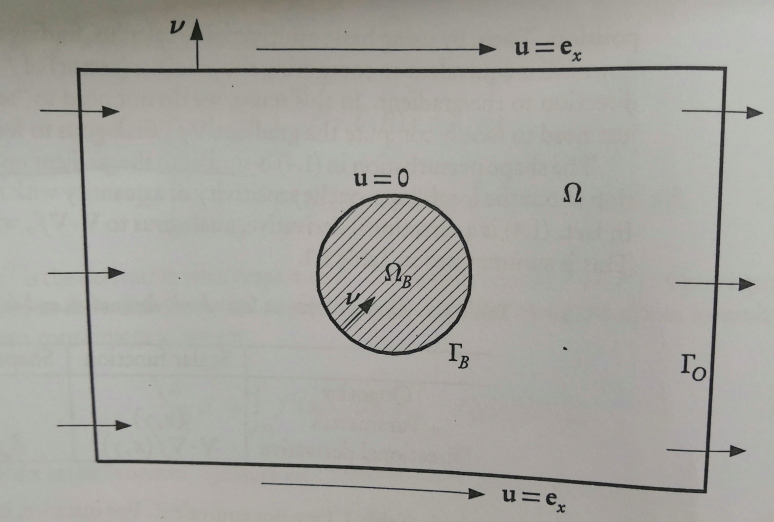
\includegraphics[scale=0.5]{./figures/11.png}
\caption{流体通过刚性$\Omega _B$ 的图。流体在$\Omega$中出现,由Navier-Stokes方程控制。$\Omega$的边界,记为$\partial \Omega$,划分为$\partial \Omega = \Gamma _B \cup \Gamma _O$,$\Gamma _B$ 为刚体的边界,$\Gamma _O$为远离刚体的外边界。$\Omega$的单位外法向量为$\nu$。}
\end{figure}

这里的目标是找到最佳形状的$\Omega _B$,以尽量减少对身体的阻力;这是形状优化中的一个经典问题$[42,69,82 -84]$。为此,我们需要指定一个形状函数代表阻力,即,
\begin{gather}
J_d(\Omega)=-e_x \cdot \int_{\Gamma _B}~\sigma(\mathbf{u},p)\nu,
\end{gather}
其中,我们使用$\Omega$来表示$\Omega _B$的形状,(这是因为$\Omega$和$\Omega _B$共享边界$\Gamma _B$。也可以证明$J_d$等于
\begin{gather}
J_d(\Omega)=\frac{1}{2Re}\int _{\Omega}\left| D(\mathbf{u}) \right|
\end{gather}
表示在$\Omega$域中能量的粘性耗散总量(单位时间)。注意,很明显,$J_d \geq 0$。利用形状扰动机制,$\delta J_d(\Omega;\mathbf{V})$表明$J_d$改变当我们在方向$\mathbf{V}$上扰动$\Omega$。因此,我们可以使用这些信息来微小的改变$\Omega$,慢慢变成一个形状,具有更好的(低级)阻力特性。

图$1.2$给出了一个数值计算来说明这一点。令$\Omega ^0$和$\Gamma _B$的初始猜测的形状的身体;这些在迭代$0$中显示。可以看到在身后面出现了两个大的涡流,这表明有大量的粘性耗散(大阻力)。优化过程,对于$\mathbf{V}$的许多不同的选择计算得到$\delta J_d(\Omega;\mathbf{V})$,至多选择一个驱动向下的$J_d$,最多。这个$\mathbf{V}$的选择用于在第一次迭代中将$\Gamma _B^0$变形为一个新的形状$\Gamma _B^1$,$\Gamma _B^0$在$\Gamma _B^1$和之间只有很小的差别。这个过程重复多次,结果如图$1.2$所示。注意旋涡(vorticses)是如何被更细的形状所消除的;显然,迭代$60$次时的对象比初始圆形具有更小的阻力。 
\begin{figure}[H]
\centering
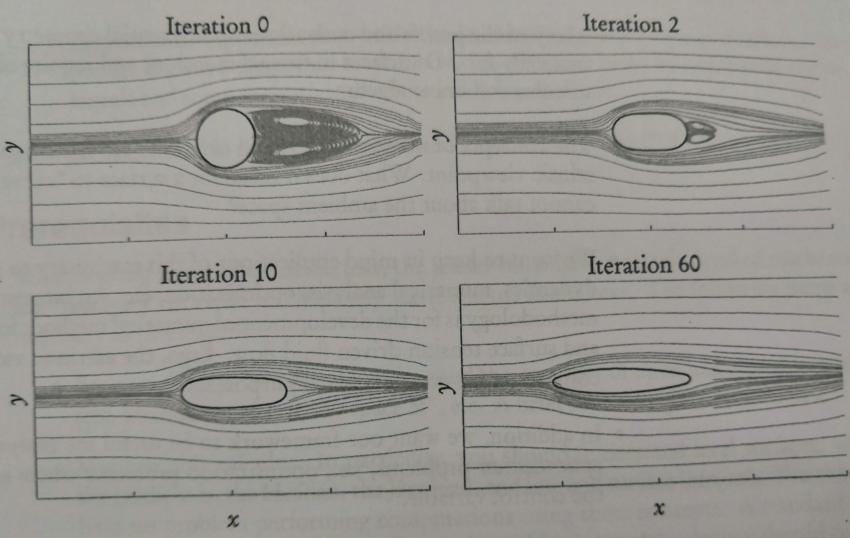
\includegraphics[scale=0.5]{./figures/12.png}
\caption{通过图形优化阻力。从一个圆形的$\Gamma _B$(不是很符合空气动力学)开始,我们应用了一个最陡的下降优化方案来缓慢地进化到最小的$J_d$。蓝色曲线是速度场$\mathbf{u}$的流线,它满足$Re=200$的$(1.5)$
}
\end{figure}

因此,形状扰动使我们能够在无限维的形状中“爬下山”。这是一个自动生成复杂工程设计的强大工具。在图$1.2$中,这是在没有人决策干涉的优化模型。在创建仅有人类干涉的$1.5$的计算机模型,开发了一种生成形状序列的优化算法。
事实上,相同的优化机制可以用于不同的PDE系统,如弹性。描述形状优化的完整细节超出了本书的范围,但是在$6.3.1$节中有一个简短的讨论

\subsection{概念}
\subsubsection{向量}
所有向量变量都被认为是列向量,并以黑体符号表示。例如,$(q_1,...,q_n)$是$\mathbb{R}^n$中一个有$n$元素的行向量。如果$\mathbf{a}\in \mathbb{R}^n$是一个列向量,则我们可以写$\mathbf{a}=(a_1,a_2,a_3)^T$,此处$T$为转置算子。两个向量的点积可以写成$\mathbf{a} \cdot \mathbf{b}=\mathbf{a}^{T} \mathbf{b}$,其中两个向量为列向量。我们定义$|\mathbf{a}|$是向量$\mathbf{a}$的欧几里得范数。附录$A$中有关于向量,矩阵的基本概念和特性。
\subsubsection{梯度}
我们使用$t$是一个曲线参数,但是有时候类似于物理时间。对于曲面,用$s_1$,$s_2$表示参数变化量。符号$\Delta$是标准空间的梯度算子。所有向量导数算子(例如$\Delta$)都被认为行向量。如果$f=f(x,y,z)$是一个标量值函数,则$\Delta f$是一个$1\time 3$行向量。符号$\Delta _x$是关于变量$\mathbf{x}$的梯度,例如$\mathbf{x}=(x,y,z)$,则
$$
\\Delta _x=\left( \frac{\partial}{\partial x},\frac{\partial}{\partial y} ,\frac{\partial}{\partial z} \right).
$$
\subsubsection{积分}
我们通常使用$\Omega$作为$\mathbb{R}^3$中体积为正的定义域(或者$\mathbb{R}^2$)。我们定义$\Gamma$是$\mathbb{R}^3$的曲面,$\sum$是曲线。通常区域$D$s上特定映射表示$id_D$,例如$id_{\Omega}(\mathbf{x})=\mathbf{x}$,对$\Omega$中所有的$\mathbf{x}$,则
$\int _{\Omega} f(\mathbf{x})\mathrm{d}\mathbf{x}=\iiint_{\Omega} f(x_1,x_2,x_3)\,\mathrm{d}x_1\,\mathrm{d}x_2\,\mathrm{d}x_3.$
$\mathrm{d}\mathbf{x}$是体积积分,$\mathrm{d}S(\mathbf{x})$是面积积分,$\mathrm{d}a(\mathbf{x})$是曲线积分。此外,我们经常写积分如下
$$
\int _{\Omega} f(\mathbf{x})\mathrm{d}\mathbf{x} \equiv \int _{\Omega} f,~~~\int _{\Gamma} f(\mathbf{x})\mathrm{d}S(\mathbf{x}) \equiv \int _{\Gamma} f,~~~\int _{\sum} f(\mathbf{x})\mathrm{d}a(\mathbf{x}) \equiv \int _{\sum} f
$$
我们定义一个集合测度$|\cdot|$,例如
\begin{gather}
|\Omega|=\int _{\Omega}1,~~~|\Gamma|=\int _{\Gamma}1,~~~|\sum|=\int _{\sum}1
\end{gather}
因此,$|\Omega|$表示$\Omega$的体积,$|\Gamma|$表示$\Gamma$的表面积,$|\sum|$表示$\sum$的长度。




\section{第二章~~~~~~~曲面和微分几何}

微分几何是对曲面(流形)形状的详细研究,包括局部和全局性质。$\mathbb{R}^3$(三维)中的平面是一个非常简单的曲面,不需要特殊的工具来描述它。另一方面,一个“任意”形状的表面,如汽车的引擎盖,有许多明显的几何特征。(高度弯曲区域、几乎平的区域等)。定量和定性地描述这些特征需要微分几何的工具。此外,几何细节在许多物理和生物过程中都很重要,例如表面张力$[20,21]$和生物膜$[9,55,90,114]$。

微分几何的框架首先通过定义一个局部映射(如,曲面参数)。然后,在曲面上建立了一个类似于标准“欧几里德微积分”的微积分框架。也可以采用其他方法,例如使用由级别集(level sets)和距离函数定义的隐式曲面。尽管是任意的,但是参数化在各种设置中都非常有用,所以我们将主要使用这些。我们强调曲面的几何形状不依赖于特定的参数化;在$2.3$节中引入正则曲面的概念来处理这个问题(参见命题$1$)。
在这一章以及本书的其余部分,我们主要关注三维空间中的二维曲面。我们首先回顾一些基础知识,以便使本文尽可能完整。

\subsection{预备}
下面几节将快速回顾本书的基本概念。然而,为了阅读本书,理解集合、映射等的所有细节并不重要。但是,如果这里讨论的观点与您完全不同,那么我们鼓励您参考一本好的教科书,如[61,62,64]
\subsubsection{欧几里得空间}
$\mathbb{R}^n$表示$n$维欧氏空间。在整个文本中,我们主要取$n=3$,但有时我们可能会专门化成$n=2$。我们假设读者熟悉笛卡尔坐标系、向量符号和向量算法、向量运算点积、叉乘、两个向量之间的夹角等。$\mathbb{R}^3$中的一般向量$\mathbf{x}$通常有由$\mathbf{x}= (x_1, x_2, x_3)$表示。

接下来,假设我们有一个给定的坐标系。任何点$P$在$\mathbb{R}^n$中都有一个唯一的位置向量,即$\mathbf{x}_P\in \mathbb{R}^n$,它从原点到$P$。点$P$的坐标就是向量$\mathbf{x}_P$的分量。因此,有时用向量$\mathbf{x}_P$来表示点$P$是很方便的,这意味着我们将通过位置矢量来表示该点。这种情况下,我们将去掉下标,只引用点$\mathbf{x}$。当没有歧义的时,我们将充分使用这种符号。否则,我们将强调点和位置向量之间的区别。
\subsubsection{开闭集合,边界,领域}
一般来说,集合是不同对象的集合。例如,$\lbrace  X,Y \rbrace$是由不同的对象$X$和$Y$组成的集合;我们在定义一个集合时使用大括号$\lbrace  , \rbrace$。我们经常引入另一个符号,如$Q=\lbrace X , Y \rbrace$,为了方便引用集合。设$S$和$U$为集合,它们之间存在关系有交集,补集,并集等。

有时候一个集合是通过一个条件定义的。例如,$ \lbrace x\in G$:$x$要满足条件$\rbrace$,例如集合$\lbrace 1,2,3\rbrace$也可以由$\left\{ a \in \mathbb{Z}:a>0~and~a<4  \right\}$定义,其中$\mathbb{Z}$是整数集。空集表示为$\emptyset $,是唯一一个没有元素的集合:$\lbrace  ~ \rbrace$。

给定$\mathbb{R}^n$中一个点$\mathbf{x}$,和一个正数$r$,设$B_r(\mathbf{x})$是$\mathbb{R}^n$中所有到点$\mathbf{x}$的距离严格小于$r$的集合,表达如下
\begin{gather}
B_r(\mathbf{x})=\left\{ \mathbf{y} \in \mathbb{R}^n:\left| \mathbf{x} - \mathbf{y} \right| <r \right\}
\end{gather}
换句话说,$B_r(\mathbf{x})$是一个以$\mathbf{x}$为中心半径为$r$的实心球($n$维)的内部。接下来,我们定义$B_r(\mathbf{x})$的边界为
\begin{gather}
\partial B_r(\mathbf{x})=\left\{ \mathbf{y} \in \mathbb{R}^n:\left| \mathbf{x} - \mathbf{y} \right|=r  \right\}
\end{gather}
即$\partial B_r(\mathbf{x})$是以$\mathbf{x}$为中心半径为$r$的球面。
从上面我们可以看到$B_r(\mathbf{x}) \cap \partial B_r(\mathbf{x})$是空集,$B_r(\mathbf{x})$不包含$\partial B_r(\mathbf{x})$的任何部分。换句话说,$B_r(\mathbf{x})$不包含其边界的任何部分。更正式的写法是$B_r(\mathbf{x}) \cap \partial B_r(\mathbf{x})=\emptyset$。

我们使用术语$open$表示一个集合不包含其边界的任何部分。更准确地说,一个子集$U$在$\mathbb{R}^n$是开的,如果$U$中每个点都有$B_r(\mathbf{x})$,其中$r>0$,且包含在$U$中。换句话说,给开集$U$中一点$\mathbf{x}$,我们可以找到一个包含$\mathbf{x}$的球完全包含在$U$中。事实上,我们经常把$B_r(\mathbf{x})$看成一个开球。另一个开放集的例子是$(0,1)\subset R$ 。 即$0$和$1$之间的组数,但不包括$0$和$1$。

一个$S\in \mathbb{R}^n$的集合的边界是$\mathbb{R}^n$中的点,使得包含此点的开集即包含有$S$中的点又包含有不是$S$中的点。换句话说,$S$中边界点$\mathbf{x}$,对于任意$r$,都满足$B_r(\mathbf{x}) \cap S\neq \emptyset$和$B_r(\mathbf{x}) \cap (\mathbb{R}^n \ S)\neq \emptyset$。我们用$\partial S$表示$S$的边界,参见图$2.1$的图形说明。
\begin{figure}[H]
\centering
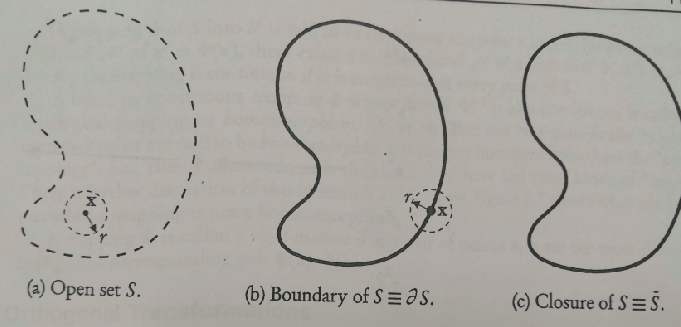
\includegraphics[scale=0.5]{./figures/21.png}
\caption{}
\end{figure}

我们用闭的说明集合包含所有边界,沿着这些线,用$\bar{S}$表示$S$的闭包,等于$\bar{S}=S \cup \partial S$。因此我们有一个以$\mathbf{x}$为圆心,半径为$r$闭合球$\overline{B_r(\mathbf{x})}$表示为
\begin{gather}
\overline{B_r(\mathbf{x})}=\left\{ \mathbf{y} \in \mathbb{R}^n:|\mathbf{x}- \mathbf{y}| \leq r \right\}
\end{gather}
另一个闭集例子$[0,1]\subset \mathbb{R}$,这个闭集即包含$0$到$1$之间的数,又包含$0$和$1$。

\textbf{备注2.}在这本书中,我们经常围绕一个点来定义一个领域,如,点$\mathbf{x}$的邻域,是任何包含$\mathbf{x}$的开集$U \subset \mathbb{R}^n$。

\subsubsection{紧集}
如果一个集合包含在$\mathbb{R}^n$中一个足够大但半径有限的开球中,那么它就是有界的。此外,如果$\mathbb{R}^n$中的集合是闭的和有界的,那么它就是紧集。紧性的概念实际上比这更普遍[63,64]。但是对于我们的目的,前面的定义是充分的。

如果$\bar{S} \subset W$和$\bar{S}$是紧的,我们说一个(非空)开集$S$紧包含在另一个开集$W$中,记为$S \subset \subset W$。也就是说,$S$的边界不能与$W$的边界接触,即,在$\partial S$和$\partial W$之间有“一点空间”。有了这个,我们现在可以证明紧支撑函数的概念。假设$f$是定义在$S$上的函数,$f$的支撑被定义为$S$中$f$的函数值非零的点的集合。
$$supp (f)= \left\{ \mathbf{x} \in S :f(\mathbf{x}) \neq 0 \right\}$$
此外,如果$\overline{supp (f)} \subset \subset S$,我们就说$f$是$S$中紧支撑。
\begin{figure}[H]
\centering
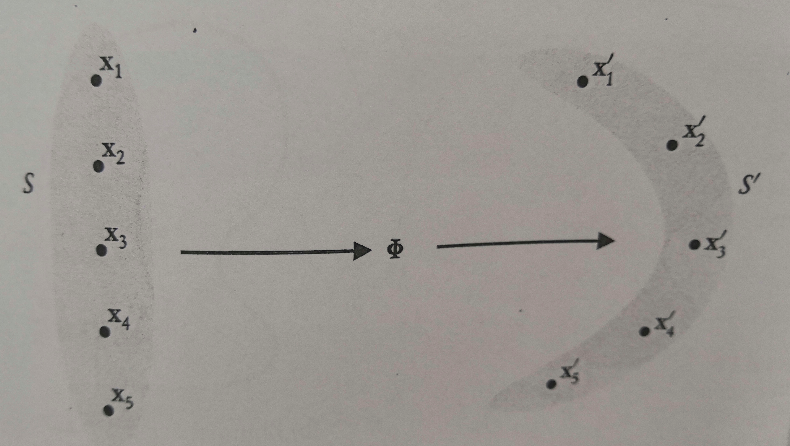
\includegraphics[scale=0.5]{./figures/22.png}
\caption{$\mathbb{R}^n$中的集合$S$通过映射$\Phi$映射到$S^{'}$上。对于$i=1,...,5$这些点对应于$\mathbf{x}_i^{'}=\Phi(\mathbf{x})$。我们可以把$\Phi$的作用解释为集合$S$变形为$S^{'}$,也就是说,$S$通过变换$\Phi$变成$S^{'}$的形状。}
\end{figure}

\textbf{备注3.}紧支持是忽略边界的有用影响。对于本书中的一些证明,我们需要这个概念来保持“一个泛函的作用”远离一个集合的边界,或者在一个感兴趣的区域内局部化一个函数。一个原因是为了避免在定义的边界上函数进行微分会产生潜在的差异。或者,更常见的是,我们希望忽略一个依赖于函数在边界点的值的量。例如,如果$f$在$S$上有紧支撑,则$\int _{\partial S}f=0$。

\subsubsection{映射:基本定义}
$S$和$S^{'}$是两组集合。如果有一个“规则”(函数)$\Phi$,使$S$中的每一点都有$S^{'}$中的点$\mathbf{x}^{'}$与之对应,则我们说这是一个集合$S$到$S^{'}$的映射或变换。我们使用符号$\Phi$:$S\rightarrow S^{'}$表达前面语句的简称。
有了这个,我们可以写成$\mathbf{x}^{'}=\Phi (\mathbf{x})$我们称$\mathbf{x}^{'}$为$\mathbf{x}$的像点,$\mathbf{x}$称为$\mathbf{x}^{'}$的逆像点。

\textbf{备注4.}一般来说,如果$S\subset \mathbb{R}^m$和$S^{'}\subset \mathbb{R}^n$,则
\begin{gather}
\Phi =(\Phi _1,\Phi _2,...,\Phi_n)^T
\end{gather}
其中每个$\Phi _i$是一个$m$个参量的函数:$\Phi _i = \Phi _i(x_1,x_2,...,x_m)$。

$S$中所有点的像点集合称为$S$的像,记为$\Phi (S)$。如果$S^{'}$中每一点都是$S$中的像点,则映射$\Phi$将$S$映到$S^{'}$上,即$S^{'}=\Phi (S)$
。在这种情况下,我们称$\Phi (S)$为满射。参见图$2.2$是$\mathbb{R}^2$中的点集映射的一个例子(参见图$2.3$是$\mathbb{R}^3$一组映射的例子)。

如$S$中任意一对不同点的像点也是$S^{'}$中的不同点,那么我们称$\Phi (S)$是单射(也叫一对一映射)。$\Phi$即是满射又是单射(称为双射),则存在$\Phi$的逆映射,记$\Phi ^{-1}$,将$S^{'}$中的点映射到$S$上。即如果$\mathbf{x},\mathbf{x}^{'}$满足$\mathbf{x}^{'}= \Phi (\mathbf{x})$,则$\mathbf{x}=\Phi ^{-1} (\mathbf{x}^{'})$,$\Phi ^{-1} :S^{'}\rightarrow S$

$S$到$S^{'}$的映射$\Phi$在$S$中的$\mathbf{x}$点处是连续的,如果对于任意包含$\mathbf{x}^{'}= \Phi (\mathbf{x})$的一个领域$N^{'}$,存在$\mathbf{x}$的一个领域$N$,使得$\Phi (N)\subset N^{'}$。如果它在$S$的每一点都是连续的,我们称该映射是连续的。

双射$\Phi$是连续映射,并且其逆$\Phi^{-1}$也是连续的,则称为拓扑映射或同胚。点集可以拓扑地互映射到其他点集称他们为同胚的。同胚集合具有相同的“拓扑”,即,它们的连通性是一样的;它们有相同类型的“洞”。在$2.3.1$节中对此有进一步的讨论,图$2.7$显示了当映射不是同胚时可以发生什么。

如果任意两点$\mathbf{a}$和$\mathbf{b}$的距离等于$\Phi(\mathbf{a})$和$\Phi(\mathbf{b})$的距离,映射$\Phi$就称为刚性运动(rigid motion)。

\subsubsection{正交变换}
设$b = (b_1, b_2, b_2)\in~\mathbb{R}^3$,$A\in~\mathbb{R}^{3\times 3}$,即一个$3\times 3$矩阵$A=[a_{ij}]_{i,j=1}^3$,$a_{i,j}$是矩阵$A$的元素。定义以下(仿射affine)线性映射$\Phi$(转换):
\begin{gather}
\tilde{\mathbf{x}}=\Phi (\mathbf{x})=A\mathbf{x}+b~~~~~~~~\Leftrightarrow~~~~~~~~\tilde{x_i}=\Phi (\mathbf{x})_i=\left( \sum _{k=1}^{3}a_{ik}x_{k} \right)+b_i,
\end{gather}
这里$(\Phi(\mathbf{x}))_i\equiv \Phi _i(x_1,x_2,x_3)$。如果$A$满足下面性质
\begin{gather}
A^{-1}=A^{T},~~~~~~~~~det(A)=1,
\end{gather}
其中$det(A)$为$A$的行列式,则$\Phi$表示刚体运动。基本上,$\Phi$由一个旋转(rotation)($A$),后跟一个转变(translation)($b$)。一个刚性运动可以被用来从一个笛卡儿坐标系统转换到另一个坐标系。

如果$b=0$并且$(2.6)$仍然成立,则$\Phi(\mathbf{x})=A\mathbf{x}$是一个线性映射称为正交变化(direct orthbogonal transformation)。这不过是以原点为中心的坐标系的旋转。如果$(2.6)$被替换为
\begin{gather}
A^{-1}=A^{T},~~~~~~~~~det(A)=-1,
\end{gather}
则$\Phi(\mathbf{x})=A\mathbf{x}$称为反正交变换,$(2.6)$和$(2.7)$都是正交矩阵的。\\

\textbf{备注4(转换的解释).}我们可以用两种不同的方法来解释$(2.5)$。考虑$\\mathbb{R}^3$坐标为$\mathbf{x}$的点$P$。\\

$\bullet$Alias.将$(2.5)$作为坐标的变换,$\mathbf{x}$和$\tilde{\mathbf{x}}$是相对于不同坐标系同一个点的坐标。换句话说,该点由不同的“名称”。\\

$\bullet$Alibi.将$(2.5)$看成集合的映射,$\mathbf{x}$和$\tilde{\mathbf{x}}$是同一坐标系下不同点的坐标。换句话说,点$\tilde{\mathbf{x}}$是点$\mathbf{x}$映射之前的点。

质点(material)的概念与alibi的观点直接相关,我们可以想象一个物质的“粒子”(即质点),最初在$\mathbf{x}$,然后因为某种物理过程而转移到$\tilde{\mathbf{x}}$点。转换$(2.5)$简单地表示物理过程的运动结果。在变形连续介质力学中是标准概念,尤其是非线性弹性力学中。图$2.3$是$\mathbb{R}^3$中点集的一个刚体运动。

\begin{figure}[H]
\centering
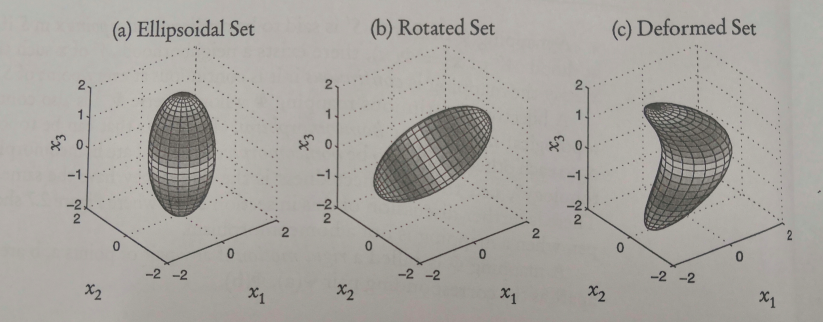
\includegraphics[scale=0.5]{./figures/23.png}
\caption{$(a)$是$\mathbb{R}^3$中点集$S$。$(b)$是$S^{'}=\Phi (S)$的旋转集合,其中$\Phi$是$(2.5)$和$(2.6)$中定义的。$(c)$是$S^{'}=\Phi (S)$的变形集合,其中$\Phi$是$(2.9)$中定义的。}
\end{figure}

\subsubsection{一般的变换}
一般来说,变换可能不是线性的。因此,$\Phi$:$\mathbb{R}^3 \Rightarrow \mathbb{R}^3$可能写成
\begin{gather}
\Phi=(\Phi _1,\Phi _2,\Phi _3)^T,
\end{gather}
这里,$(\Phi_i= \Phi _i(x_1,x_2,x_3) (i = 1,2,3)$为标量值(非线性)函数。备注$5$也适用于这些转换。因此,alias的观点生成一个曲线坐标系。alibi观点意味着集合$S$变形为$S^{'}=\Phi (S)$。如图$2.3$所示,非线性映射被应用于椭球形点集的例子,其中$\Phi$定义为
\begin{gather}
\Phi=(x_1-1.2+1.6\cos (x_3 \pi /4),x_2,x_3)^T.
\end{gather}

当处理从$\mathbb{R}^n$映射到$\mathbb{R}^n$的变换时,我们将使用符号$\Phi$来表示变换(通常$n =2$或$3$),但是我们也将考虑从$\mathbb{R}^q$到$\mathbb{R}^n$的变换,其中$q <n$。当$q = 2$和$n = 3$时,我们用转换$X$:$\mathbb{R}^2 \Rightarrow \mathbb{R}^3$,我们使用不同的符号去表示;在定义曲面时使用这(参见$2.2.1$和$2.3$节)。注意,我们可以把$X$看作$\Phi$是对$x_1,x_2$平面的限制。当$q = 1$时,我们使用符号$\alpha$:$\mathbb{R}^1 \Rightarrow \mathbb{R}^n$,$n=2,3$,这对应于参数化曲线。类似地,我们可以把$\alpha$看成是$\Phi$对$x_1$轴的限制。
\subsection{参数方法}
\subsubsection{什么是曲面}
曲面是空间中非常有规律(regular enough)的一组点。空间中点的随机分散不符合我们对曲面的直观概念。例如,它不够规律。另一方面,球面的边界确实符合我们对曲面的概念,也就是说,由于球面是“光滑的”,所以它具有足够的规律来作为曲面。
\begin{figure}[H]
\centering
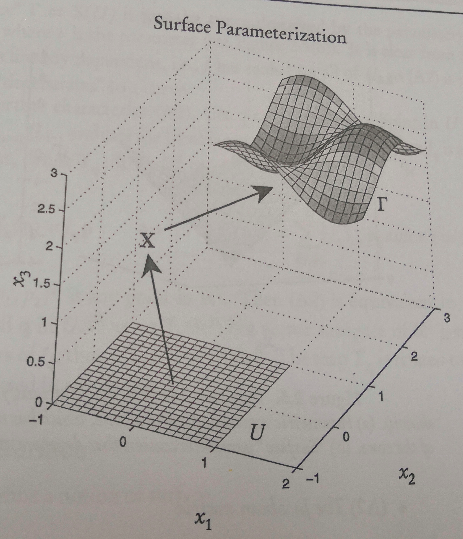
\includegraphics[scale=0.5]{./figures/24.png}
\caption{参数表示的例子。参考域$U$是$x_1,x_2$平面上的方形显示。映射$X$将集合$U$对应于曲面$\Gamma$(曲面基于$x_3$坐标着色)。}
\end{figure}

直观地说,我们可以把创建一个表面想象成把一个平的橡胶板变形成一个弯曲的板。第$2.1.6$节中的变换$X$捕捉到了这个思想。因此,令$U \subset \mathbb{R}^2$是一个“平”域,令$X$:$U\Rightarrow \mathbb{R}^3$是个变形变换,例如,对于$U$中的每一个点$(s_1,s_2)^T$都对应于$\mathbb{R}^3$的点$x= (x_1,x_2, x_3)^T$使得
\begin{gather}
\mathbf{x}=X(s_1,s_2).
\end{gather}
令$\Gamma=X(U)$表示由“变形”$U$得到的曲面。我们称$(2.10)$是曲面$\Gamma$的参数表示,其中$s_1,s_2$称为表达参数。有时,我们把$U$作为一个参考域。有关$(2.10)$的示例,请参见图$2.4$。\\
\textbf{允许参数化}\\
如果我们要用$(2.10)$来定义曲面,那么我们必须对$X$进行假设,以保证$\Gamma=X(U)$是一个有效的曲面。最起码,X必须是连续的,以避免“撕裂”橡胶板。但是如果我们想对$\Gamma$做微积分,我们实际上需要更多。\\
\textbf{假设1.}我们对$X$做如下规律性假设。\\
$\bullet$ $(A1)$函数$X(x_1,x_2)$在$U$上是$C^{\infty}$,$\Gamma$中的每个点$\mathbf{x} = X(s_1,s_2)$对应于$U$中的一个点$(s_1, s_2)$,$X$是单射。
\begin{figure}[H]
\centering
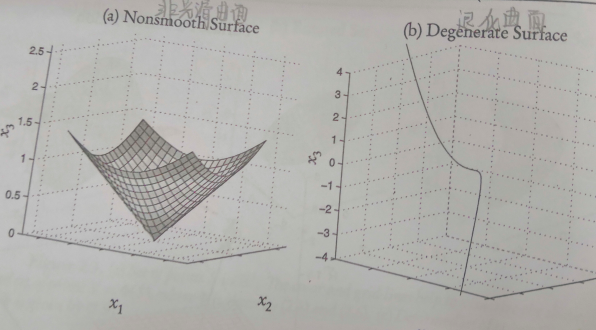
\includegraphics[scale=0.5]{./figures/25.png}
\caption{这里的例子不满足假设$1$(参考域$U$没有显示)。$(a)$是一个圆锥体的参数表达,它在圆锥体的角上不能定义切平面。$(b)$是一个曲线,退化的曲面}
\end{figure}
$\bullet~(A2)$雅克比行列式(Jacobian)在$U$上秩为$2$,$J$ 的列向量是线性无关的。
\begin{gather}
J=\left[ \partial _{s_1}X,\partial _{s_2}X \right]=
\begin{bmatrix}
\partial _{s_1}X_1  & \partial _{s_2}X_1 \\
\partial _{s_1}X_2  & \partial _{s_2}X_2 \\
\partial _{s_1}X_3  & \partial _{s_2}X_3 
\end{bmatrix}
\end{gather}

我们说方程$(2.10)$的参数满足$(A1)$和$(A2)$是参数化的,用更现代的话说,immersion
\textbf{重要性}\\
假设$(A1)$对平面施加了一定的光滑性,即在$\Gamma$中的每一点上都有定义良好的切平面。切平面的精确定义见第$2.4.3$节;现在,我们只需要一个切平面的直观概念。例如,令$U=(-1,1)\times (-1,1)$并且考虑映射
\begin{gather}
X(s_1,s_2)=(s_1,s_2,\sqrt{s_1^2+s_2^2})^T~~~~~~~~(s_1,s_2)^T\in U.
\end{gather}
曲面$\Gamma = X(U)$是一个圆锥(见图$2.5(a)$)。很明显,$(2.12)$在$(0,0)^T$处不可导,即$(A1)$是无效的。因此,不存在唯一通过$(0,0,0)^T$且与表面$\Gamma$“相切”的平面。

需要假设$(A2)$来避免集合$\Gamma$(由$(2.10)$参数化)为$\mathbb{R}^3$中的曲线的可能性。通过线性代数,$A(2)$等价于$\partial _{s_1}X \times \partial _{s_2}X\neq 0$,这也等价于在$\mathbb{R}^3$中$\partial _{s_1}X$和$\partial _{s_2}X$是线性无关的向量。例如,令$U= (-1,1) \times (-1,1)$并且考虑映射
\begin{gather}
X(s_1,s_2)=(s_1+s_2,(s_1+s_2)^2,(s_1+s_2)^3)^T~~~~~~~~(s_1,s_2)^T\in U.
\end{gather}
“曲面”$\Gamma =X(U)$就是通过$X(t)=(t,t^2,t^3)^T$参数化后的曲线,其中t为参数(见图$2.5(b)$)。由$(2.13)$可知,$\partial _{s_1}X$和$\partial _{s_2}X$是线性相关的,即,在所有$U$上秩都是1,所以$(A2)$ 无效。因此,表面“退化”成曲线。

我们进一步描述$(A2)$。令$\mathbf{q}=(q_1,q_2)^T$为$U$中的一个点,定义$J^{q}=\left[ \partial _{s_1}X,\partial _{s_2}X \right]|_{s=q}$,(求出该点的雅可比矩阵)。注意$J_p$是$\mathbb{R}^{3\times 2}$中的一个常数矩阵。接下来,定义$T_q:\mathbb{R}^2 \Rightarrow \mathbb{R}^3$
\begin{gather}
T_q(\mathbf{p})=J_q \mathbf{p}~~~~~~~\Leftrightarrow~~~~~~~(T_q(\mathbf{p}))_i=\sum_{k=1}^{2}(J_q)_{ik}p_k~~~i=1,2,3,
\end{gather}
其中$\mathbf{p}= (p_1,p_2)$是$\mathbb{R}^2$中的任意一点。那么$(A2)$等价与映射$T_q$,是$U$中所有$\mathbf{q}$单射。集合$T_q(\mathbb{R})^2$是$J_q$中两个列向量产生;因此,它的维数是$2$。映射$T_q$与切平面有关,这将在$2.4.3$节中讨论。

\subsubsection{曲面参数化}
现在我们可以定义曲面的概念。

\textbf{定义1(参数曲面)}。令$U \subset \mathbb{R}^2$是一个开集并且考虑一个映射$X:\Rightarrow \mathbb{R}^3$。如果$X$在$U$中是可微的,我们称$(U,X)$是一个参数曲面。如果映射$T_q$对于所有$U$中的$\mathbf{q}$是单射,则称$X$是正则的(regular)。此外,如果有一个$U$中的$\mathbf{p}$不是单射,或未定义,则我们称$\mathbf{p}$时$X$的一个奇异点;否则,这是一个正则点。\\

注意,我们将这对$(U,X)$称为参数曲面,因为$\Gamma=X(U)$是构成曲面的点集,$U$和$X$描述了如何在$\Gamma$上“绘制”坐标曲线。进一步阐述可以见图$(2.4)$。参考域$U$只是组成一个正方形的一组点。然而,$U$上的网格线对应于$U$上的坐标系统,这些网格线通过$X$映射到$\Gamma$(见图$2.4$),这定义了$\Gamma$上的一种曲线坐标系。

如果我们在$U$上选择了一个不同的坐标系,那么网格线在$U$(和$\Gamma$)上看起来就会不一样。在$\Gamma$上会有一个不同的曲线坐标系(参见图$2.10$)。

因此,曲面可以以多种方式参数化就不足为奇了。实际上,给定$\Gamma$的一个参数化$(U,X)$
\begin{gather}
s_1=s_1(\tilde{s}_1,\tilde{s}_2),~~~s_2=s_2(\tilde{s}_1,\tilde{s}_2),~~~(\tilde{s}_1,\tilde{s}_2)^T \in ~\tilde{U}
\end{gather}
即,$s:\tilde{U} \rightarrow \mathbb{R}^2$和$U=s(\tilde{U})$。接下来,定义$\tilde{X}=X\circ s$,意味着
$$\tilde{X}(\tilde{s}_1,\tilde{s}_2)=X(s_1(\tilde{s}_1,\tilde{s}_2),s_2(\tilde{s}_1,\tilde{s}_2)).$$
这里$(\tilde{U},\tilde{X})$也是$\Gamma$的一个参数化。可以把$s$当成$\tilde{U}$到$U$的映射($s^{-1}$看成$U$到$\tilde{U}$的映射)
\begin{figure}[H]
\centering
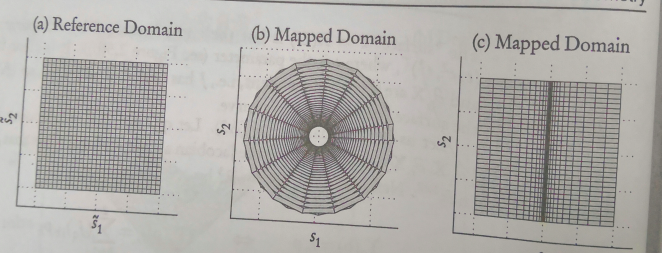
\includegraphics[scale=0.5]{./figures/26.png}
\caption{所示图是不满假设$2$的例子。$(a)$是参考域。$(b)$是使用$(2.17)$中的映射$U$映射到一个环,注意这个环面覆盖了两次。$(c)$是使用$(2.18)$中的映射$U$映射到一个方形。网格线在$s_1$的附近挤压在一起}
\end{figure}

当然,为了有一个正则的参数化,我们必须有假设$1$必须满足$(\tilde{U},\tilde{X})$。这需要对$(2.15)$做以下假设。\\
\textbf{假设2.}\\
$\bullet~(A0*)$方程$(2.15)$被定义在区域$\tilde{U}$上且使得$U=s(\tilde{U})$。\\
$\bullet~(A1*)$方程$(2.15)$在$\tilde{U}$上是$C^{\infty}$,并且它是单射的。\\
$\bullet~(A2*)$雅克比矩阵
\begin{gather}
D=\left[ \partial _{\tilde{s}_1}s,\partial _{\tilde{s}_2}s \right]=
\begin{bmatrix}
\partial _{\tilde{s}_1}s_1  & \partial _{\tilde{s}_1}X_1 \\
\partial _{\tilde{s}_1}s_2  & \partial _{\tilde{s}_2}X_2 
\end{bmatrix}
\end{gather}
对于$\tilde{U}$上所有点$(\tilde{s}_1,\tilde{s}_2)$是非奇异的,即在$\tilde{U}$上$det(D)\neq 0$

我们说形如满足假设$2$的$(2.15)$的变换是一个允许的坐标变换(allowable)。

条件$(A1*)$和$(A2*)$彼此完全独立,实际上
\begin{gather}
s_1=e^{\tilde{s}_1}\cos (2\pi \tilde{s}_2),~~~~~s_2=e^{\tilde{s}_1}\sin (2\pi \tilde{s}_2)
\end{gather}
当$-1 \leq \tilde{s}_2 \leq 1$时是非单射的变换;然而,一个简单的计算给出$det(D) = (2\pi)^2e^{2\tilde{s}_2}$,它在$s_1,s_2$平面上从不为零(参见图$2.6$)。另一方面,变换
\begin{gather}
s_1=\tilde{s}^3 ,s_2=\tilde{s}
\end{gather}
处处都是单射,但是一个简单的计算得到$det(D)=3\tilde{s}_1^2=3\tilde{s}_1^{2/3}$,当$s=0$时,在整个$s_2$轴上它为零。(见图$2.6$)


\input{2.3.tex}
\subsection{连续高斯链模型}
连续高斯链是一种用于分析和数值计算的理想链模型,该模型可以被视为离散高斯链模型的连续极限,其中的聚合物被视为一个连续的线性弹性丝(linearly elastic filament)。如图2.5所示,连续高斯链的构型由空间曲线$\mathbf{r}(s)$描述,表示高分子长链上某一链节的位置,其中$s\in [0,N]$,被定义为路径(contour)变量。第$s$个链节在空间中的位置记为$\mathbf{r}(s)$,末端距矢量(end-to-end-vector)$R$可以表达为$R=\mathbf{r}(N)−\mathbf{r}(0)$。
\begin{figure}[H]
\centering
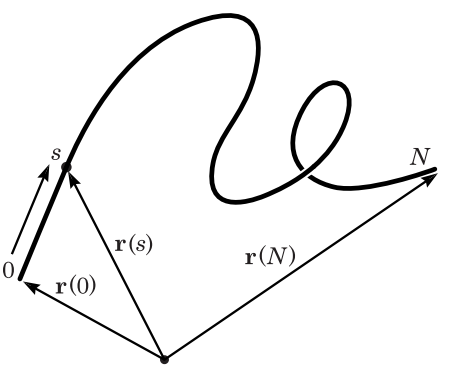
\includegraphics[scale=0.7]{./figures/41.png}
\caption{}
\end{figure}
图2.5:空间曲线$\mathbf{r}(s)$描述连续高斯链模型将聚合物的构型,其中$s\in [0,N]$是路径参数。$\mathbf{r}(0)$和$\mathbf{r}(N)$是链端位置。

连续高斯链的势能可以写成
\begin{gather}
U_0[\mathbf{r}]=\frac{3k_BT}{2b^2}\int_{0}^{N} \mathrm{d}x\left| \frac{d\mathbf{r}(s)}{ds} \right|^2
\end{gather}
其中$b$为链节的统计长度,$U_0[\mathbf{r}]$的方括号符号表示$U_0$是定义聚合物构型的空间曲线$\mathbf{r}(s)$的泛函。泛函是连续函数到数之间的映射。势能的形式与离散高斯链的方程$U_0(\mathbf b^N)=\sum_{i=1}^{N}h(\left|\mathbf{b}_i\right|^2 )$和$h(x)=\frac{3k_BT}{2b^2}x^2$密切相关。如果我们将$\frac{d\mathbf{r}(s)}{ds}$看作高分子长链上第$s$节(链节长度为$ds$)的拉伸形变,则方程$(2.42)$对链的整个路径上每一个这样的微分段的谐波势贡献(harmonic potential contribution)求和。值得注意的是,在连续高斯链模型中,$s$并不表示弧长,而只是表示链上各段的参数指标。因此,拉伸$\frac{d\mathbf{r}(s)}{ds}$不是固定单位向量,它的大小是可以自由波动。势能方程$(2.42)$通常称为“Edwards Hamiltonian”。

连续高斯链的构型配分函数可以写成
\begin{gather}
Z_0=\int \mathcal{D}\mathbf{r}~\exp(-\beta U_0[\mathbf{r}])
\end{gather}
其中$\int \mathcal{D}\mathbf{r}$表示所有可能的描述聚合物的构型的空间曲线$\mathbf{r}(s)$上的泛函积分。这类泛函积分,又称路径积分,是量子力学和概率论领域(Feynman和Hibbs,1965)所熟悉的,其中$\mathbf{r}(s)$对应于量子粒子或布朗(Brownian)粒子在时间$s$的位置。实际上,方程$(2.43)$是经典扩散(brownian motion)路径积分描述中的维纳运动(Wiener motion)。

路径积分是一种复杂的数学对象,在定义和操作上需要一定的精确性(Simon,1979)。然而在这里,我们将非正式地和以物理的方式来研究这些对象。定义路径积分有两种方法,其中一种方法是用$N_s+1$个等距路径点去离散路径,因此我们用$N_s+1$个点的空间位置逼近连续函数$\mathbf{r}(s)$,其中这$N_s+1$个点由向量$(\mathbf{r}_0,\mathbf{r}_1,...,\mathbf{r}_{N_s})$表示。这样,路径积分可以定义为$3(N_s+1)$维的普通积分(假设聚合物在体积为$V$的三维空间中)
\begin{gather}
\int \mathcal{D}\mathbf{r}\approx \prod_{i=0}^{N_s} \int \, \mathrm{d} \mathbf{r}_i
\end{gather}
其中,近似的质量随着$N_s$的增加而提高。当$N_s$有限时,连续高斯链的路径积分近似于有$N_s+1$个珠子的离散高斯链的配分函数。特别是,我们有一个近似
\begin{gather}
Z_0\approx \prod_{j=0}^{N_s} \int \, \mathrm{d} \mathbf{r}_j~\exp \left( -\frac{3}{2b^2\bigtriangleup s}\sum_{i=1}^{N_s}\left|\mathbf{r}_{i-1}-\mathbf{r}_i \right|^2 \right)
\end{gather}
其中,其中一个$N_s$键的均方长度(mean-squared)由$b^2\bigtriangleup s$给出,$\bigtriangleup s=N/N_s$是路径点之间的间距。

方程$(2.45)$的巧妙之处源于连续极限,因为$Z_0$尺度为$VN_s^{−(3/2)N_s}$,当$N_s\rightarrow \infty$时为零。通常我们对平均值感兴趣,它可以表示成两路径积分的比率。例如,连续高斯链的末端距矢量的均方值可以表示为
\begin{gather}
R^2\equiv \left \langle \mathbf{R}\cdot \mathbf{R}\right \rangle _0=\frac{\int \mathcal{D}\mathbf{r}\left| \mathbf{r}(N)-\mathbf{r}(0) \right|^2~\exp(-\beta U_0[\mathbf{r}])}{\int \mathcal{D}\mathbf{r}~\exp(-\beta U_0[\mathbf{r}])}
\end{gather}
其中分母只是配分函数$Z_0$。当根据方程$(2.45)$对上述方程的分子和分母中的路径积分进行离散时,
发现奇异因子完全抵消,从而当$N_s\rightarrow \infty$时,$R^2$更好定义。此外,在路径积分的数值计算中,通常采用有限的$N_s$来避免奇异性。

定义路径积分的另一种方法是通过路径的谱表示(spectral represention)。特别是,我们可以用扩充的一组完整的基函数$\lbrace \phi _0(s),\phi _1(s),... \rbrace$来表示空间曲线$\mathbf{r}(s)$
\begin{gather}
\mathbf{r}(s)=\sum_{p=0}^{\infty} \mathbf{a}_p \phi _p(s)
\end{gather}
这是一种广义的傅里叶展开式,其展开式系数$\mathbf{a}_p$可以看作是广义傅里叶系数(见附录A)。对于在流体介质中自由悬浮(freely suspended in a fluid medium)的聚合物,基函数的一种方便的选择是符合“无拉伸”(no-stretch)边界条件的余弦集$\frac{d\mathbf{r}(s)}{ds}\vert _{s=0}=\frac{d\mathbf{r}(s)}{ds}\vert _{s=N}=0$。这相当于余弦傅里叶级数表示
\begin{gather}
\mathbf{r}(s)=\mathbf{a}_0+2\sum_{p=1}^{\infty} \mathbf{a}_p \cos(p\pi s/N)
\end{gather}
根据这些基函数的正交性可以求解傅里叶系数
\begin{gather}
\mathbf{a}_p=\frac{1}{N}\int_{0}^{N}  \mathrm{d}x~\cos(p\pi s/N)\mathbf{r}(s),p=0,1,2,...,\infty
\end{gather}
这些模型在聚合物文献中被称为Rouse模型,在聚合物动力学理论中起着特别重要的作用(Doi和Edwards,1986)。实际上,$\mathbf{a}_0$可以解释为聚合物质心的位置,而$\mathbf{a}_p,p=1,2,3,...$,尺度越细则提供更多关于聚合物形状的信息。

利用Rouse谱表示,聚合物的所有构型(路径)上的积分可以解释为对所有Rouse模型的积分的乘积。
\begin{gather}
\int \mathcal{D}\mathbf{r}= \prod_{p=0}^{\infty} \int \, \mathrm{d} \mathbf{a}_p
\end{gather}
上述表达式右手边的对象是一个无穷维积分,所以我们再次遇到了配分函数$Z_0$的存在性问题。然而,这两个路径积分的比率证明是有限的,
为了数值计算的目的,我们取有限$P\gg1$使路径积分正则化(消除奇异点)
\begin{gather}
\int \mathcal{D}\mathbf{r}\approx \prod_{p=0}^{P} \int \, \mathrm{d} \mathbf{a}_p\end{gather}
为了说明Rouse模型在连续高斯链计算中的应用,用Rouse模型表示末端距矢量的均方值是
\begin{gather}
\left | \mathbf{r}(N)-\mathbf{r}(0) \right |^2=16\sum_{p=1,3,...}^{\infty}\sum_{q=1,3,...}^{\infty} \mathbf{a}_p \cdot \mathbf{a}_q
\end{gather}
这个数的均值可以写为
\begin{gather}
\left \langle \left| \mathbf{R} \right|^2 \right \rangle _0=16\sum_{p=1,3,...}^{\infty}\sum_{q=1,3,...}^{\infty} \left \langle \mathbf{a}_p \cdot \mathbf{a}_q \right \rangle _0
\end{gather}
其中,在Rouse模型中定义对象$f(\mathbf{a})$的平均值为
\begin{gather}
\left \langle f(\mathbf{a}) \right \rangle _0=\frac{\begin{matrix} \prod_{p=1}^{\infty} \int \, \mathrm{d} \mathbf{a}_p f(\mathbf{a})\exp(-\beta U_0(\mathbf{a})) \end{matrix}}{\begin{matrix} \prod_{p=1}^{\infty} \int \, \mathrm{d} \mathbf{a}_p \exp(-\beta U_0(\mathbf{a})) \end{matrix}}
\end{gather}
在Rouse模型表达式中,方程$(2.42)$的势能是对角的
\begin{gather}
\beta U_0(\mathbf{a})=\frac{1}{2}\sum_{p=1}^{\infty}\alpha (p)\mathbf{a}_p \cdot \mathbf{a}_p
\end{gather}
其中$\alpha (p)=6\pi ^2p^2/(b^2N)$。注意,质心$p=0$模型是均匀分布。$p>0$模型都是统计独立的,是高斯分布,因此如下有(附录B)
\begin{gather}
\left \langle \mathbf{a}_p \cdot \mathbf{a}_q \right \rangle _0=\frac{3}{\alpha (p)}\delta _{pq}
\end{gather}
替换到方程$(2.53)$将得
\begin{gather}
\left \langle \left| \mathbf{R} \right|^2 \right \rangle _0=\frac{8b^2N}{\pi ^2}\sum_{p=1,3,...}^{\infty}\frac{1}{p^2}=b^2N
\end{gather}
由此我们得出结论:连续高斯链具有离散高斯链的性质,它的末端距矢量的均方值由$R=bN^{1/2}$给出。类似用期望公式给出连续高斯链的卷积公式$R_g=b(N/6)^{1/2}$。

\begin{figure}[H]
\centering
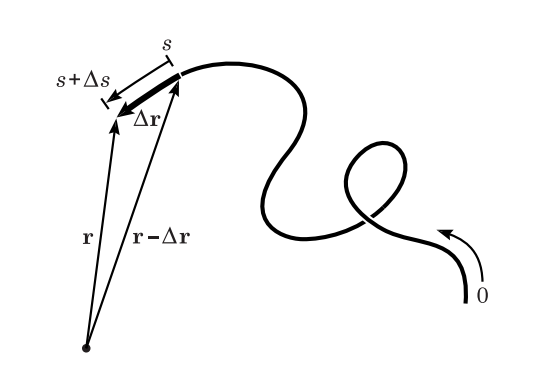
\includegraphics[scale=0.7]{./figures/42.png}
\caption{}
\end{figure}

图2.6;用“随机过程”(stochastic process)方法从具有$s$段的连续高斯链的统计权重中构造出具有$s+\bigtriangleup s$段的连续高斯链末端位置的统计权重。

在探索连续高斯链模型的性质时,我们现在回到了随机过程方法。具体来说,考虑一个约化的分布函数$p_0 (\mathbf{r},s)$是很有用的,它描述了在$\mathbf {r}$处,一个连续的路径长度为$s$的高斯链。这个函数满足归一化条件的,即$\int \, \mathrm{d} \mathbf{r}~p_0(\mathbf{r},s)=1$。通过对离散高斯链的方程$p_0(\mathbf{r},j)=\int \, \mathrm{d} \mathbf{b}_j~\Phi(\mathbf{b}_j;\mathbf{r}-\mathbf{b}_j)p_0(\mathbf{r}-\mathbf{b}_j,j-1)$的类比,我们可以通过Chapman-Kolmogorov方程利用非常小的链的信息建立分布函数
\begin{gather}
p_0(\mathbf{r},s+\bigtriangleup s)=\int \, \mathrm{d}(\bigtriangleup \mathbf{r})\Phi(\bigtriangleup \mathbf{r};\mathbf{r}-\bigtriangleup \mathbf{r})p_0(\mathbf{r}-\bigtriangleup \mathbf{r},s)
\end{gather}

图2.6说明了上述方程的物理内容,它依赖于连续链的最后一部分离散化。转移概率密度$\Phi(\bigtriangleup \mathbf{r};\mathbf{r}-\bigtriangleup \mathbf{r})$描述了路径长度$\bigtriangleup s$的链段的位移为$\bigtriangleup \mathbf{r}$的条件概率,从路径位置$s$处的$\mathbf{r}-\bigtriangleup \mathbf{r}$开始。连续高斯链的相关随机过程是稳定的,所以$\Phi =\Phi(\bigtriangleup \mathbf{r})$与起始位置和路径位置无关。$\Phi(\bigtriangleup \mathbf{r})$的表达式直接来自于连续高斯链方程$(2.45)$之前的离散化:
\begin{gather}
\Phi(\bigtriangleup \mathbf{r})=\left( \frac{3}{2\pi b^2 \bigtriangleup s} \right)^{3/2}\exp \left(- \frac{3\left| \bigtriangleup \mathbf{r} \right|^2}{2b^2 \bigtriangleup s} \right)
\end{gather}
连续链模型的一个有用的特点是,Chapman-Kolmogorov积分方程可以归结为偏微分方程,在概率论中可归结为Fokker-Planck方程(van Kampenn,1981)和量子理论中的Feynman-Kac公式(Feynman和Hibbs,1965)。我们通过导出与方程$(2.58)$相结合的Fokker-Planck方程来说明这一点。这一推导是方程的两边通过泰勒展开。注意到在这种情况下,$\Phi(\bigtriangleup \mathbf{r};\mathbf{r}-\bigtriangleup \mathbf{r})$与初始位置$\mathbf{r}-\bigtriangleup \mathbf{r}$无关,我们不扩展转移概率。有
\begin{equation}
\begin{aligned}
p_0(\mathbf{r},s)+\bigtriangleup s\frac{\partial}{\partial s}p_0(\mathbf{r},s)+O(\bigtriangleup s^2)=&p_0(\mathbf{r},s)-\left \langle \bigtriangleup \mathbf{r} \right \rangle _\Phi \cdot \triangledown p_0 (\mathbf{r},s)\\ &+\frac{1}{2!}\left \langle \bigtriangleup \mathbf{r}  \bigtriangleup \mathbf{r} \right \rangle _\Phi:\triangledown \triangledown p_0(\mathbf{r},s)\\ &+O(\left \langle \bigtriangleup \mathbf{r}  \bigtriangleup \mathbf{r}  \bigtriangleup \mathbf{r} \right \rangle _\Phi)
\end{aligned}
\end{equation}
其中,该方程中出现的$\Phi$平均定义为
\begin{gather}
\left \langle f(\bigtriangleup \mathbf{r}) \right \rangle _\Phi = \int \, \mathrm{d}(\bigtriangleup \mathbf{r})\Phi (\bigtriangleup \mathbf{r})f(\bigtriangleup \mathbf{r})
\end{gather}
利用方程$(2.59)$的显式高斯形式,可以将方程$(2.60)$右侧的平均值计算为(附录B)
\begin{gather}
\left \langle \bigtriangleup \mathbf{r} \right \rangle _\Phi = 0
\end{gather}
\begin{gather}
\left \langle \bigtriangleup \mathbf{r} \bigtriangleup \mathbf{r}_\beta \right \rangle _\Phi = \frac{b^2 \bigtriangleup s}{3}\delta_{\alpha \beta}
\end{gather}
如果我们将这些式子带入方程$(2.60)$中,则$\bigtriangleup s \rightarrow \infty$时的分布函数$p_0(\mathbf{r},s)$满足Fokker-Planck方程

\begin{gather}
\frac{\partial}{\partial s}p_0(\mathbf{r},s)=\frac{b^2}{6}p_0(\mathbf{r},s)
\end{gather}

因此,连续高斯链的Fokker-Planck方程给出的具有“扩散系数”$b^2/6$
的传统扩散方程的形式。该方程的解提供了关于端点段$p_0(\mathbf{r},s)$分布的完整信息。

Fokker-Planck方程是特别方便,因为有各种各样的分析和数值技术可用于求解偏微分方程。对于方程$(2.64)$,对应于初始条件$p_0(\mathbf{r},s)=\delta(\mathbf{r})$的基本(格林函数)解是
\begin{gather}
p_0(\mathbf{r},s)=\left[ 3/(2 \pi sb^2) \right]^{3/2}\exp \left[ -3\left| \mathbf{r} \right|^2/(2sb^2) \right]
\end{gather}
如果令$s=N,\mathbf{r}=\mathbf{R}$,则末端距矢量恢复成熟悉的高斯分布函数$(2.38)$
在比单键更大的尺度下,离散高斯链和连续高斯链明显具有相同的链端分布函数。使用连续链的优点是它允许用偏微分方程进行计算。这一优势将在第三章中变得更加明显,在第三章中,我们将考虑有外势的链。
%\endinput
\cite{tam19912d}
%\bibliography{../ref}
\end{document}
